\documentclass[aspectratio=169,11pt]{beamer}
\usetheme{default}
\usepackage[T1]{fontenc}
\usepackage{lmodern,booktabs,tabularx,graphicx,tikz}
\usetikzlibrary{arrows.meta,positioning,calc}
\definecolor{wine}{HTML}{9B1C2B}
\definecolor{orange}{HTML}{D97800}
\definecolor{cream}{HTML}{FFF9F5}
\definecolor{ink}{HTML}{302F2D}
\definecolor{muted}{HTML}{756A65}
\setbeamercolor{normal text}{fg=ink,bg=cream}
\setbeamercolor{structure}{fg=wine}
\setbeamercolor{frametitle}{fg=wine,bg=cream}
\setbeamerfont{frametitle}{size=\Large,series=\bfseries}
\setbeamertemplate{navigation symbols}{}
\setbeamertemplate{itemize item}{\color{wine}\small\textbullet}
\setbeamertemplate{footline}{\hspace{1em}\color{muted}\scriptsize TriAlign progress\hfill\insertframenumber\hspace{1em}\vspace{.5em}}
\newcolumntype{Y}{>{\raggedright\arraybackslash}X}
\newcommand{\gap}{\par\vspace{.55em}}
\newcommand{\status}[1]{{\color{wine}\textbf{#1}}}
\title{TriAlign}
\subtitle{Progress in comparing clinical trial eligibility criteria}
\author{Jonathan Ma and Jiatong Gao}
\date{November 2026}
\begin{document}
\raggedright

\begin{frame}[plain]
\vspace{.7cm}
{\Huge\color{wine}\bfseries TriAlign\par}
\gap
{\Large Progress in comparing clinical trial\\eligibility criteria\par}
\vspace{1cm}
Jonathan Ma \qquad Jiatong Gao\par
\gap
{\color{muted}November 2026}
\end{frame}

\begin{frame}{Project objective}
Help a clinician compare the eligibility requirements of Trial A and Trial B.
\gap
\begin{enumerate}
\item Align potentially corresponding criteria across the trials.
\item Explain relationships and differences using source evidence.
\item Identify criteria needing further review and preserve unresolved comparisons.
\end{enumerate}
\gap
\textbf{Illustrative case:} inclusion age $\geq18$ versus inclusion age $<18$.\\
Shared words conceal disjoint allowed populations.
\gap
Scope: trial comparison through criterion alignment, without patient screening.
\end{frame}

\begin{frame}{From extracted criteria to trial comparison}
\centering
\resizebox{.98\textwidth}{!}{%
  \IfFileExists{docs/figures/trial_comparison_workflow.tex}
    {% Shared editable diagram used by the progress deck and technical document.
\begingroup
\definecolor{wfWine}{HTML}{9B1C2B}
\definecolor{wfOrange}{HTML}{D97800}
\definecolor{wfInk}{HTML}{302F2D}
\definecolor{wfPale}{HTML}{FFF9F5}
\hyphenpenalty=10000
\exhyphenpenalty=10000
\begin{tikzpicture}[
  font=\sffamily\fontsize{10}{12}\selectfont,
  wfbox/.style={draw=wfInk!55,line width=.65pt,rounded corners=2pt,
    fill=white,text=wfInk,align=center,text width=2.8cm,
    minimum height=2.5cm,inner sep=6pt},
  wfsystem/.style={wfbox,draw=wfWine,fill=wfPale},
  wfarrow/.style={-{Latex[length=2.2mm]},draw=wfWine,line width=.9pt}
]
\node[wfbox] (trials) at (0,0) {
  \textbf{1. Select trials}\\[4pt]
  Clinician chooses\\Trial A + Trial B
};
\node[wfsystem] (extract) at (3.65,0) {
  {\color{wfWine}\textbf{2. Extracted}}\\
  {\color{wfWine}\textbf{criteria}}\\[4pt]
  Modern AutoCrit or\\another compatible source
};
\node[wfbox] (handoff) at (7.3,0) {
  \textbf{3. Review}\\\textbf{and import}\\[4pt]
  Reviewed files\\Source evidence
};
\node[wfsystem] (compare) at (10.95,0) {
  {\color{wfWine}\textbf{4. TriAlign}}\\[4pt]
  Identify pairs\\Compare clinical\\relationships
};
\draw[wfarrow] (trials) -- (extract);
\draw[wfarrow] (extract) -- (handoff);
\draw[wfarrow] (handoff) -- (compare);

\node[draw=wfOrange,line width=.8pt,rounded corners=2pt,
  fill=white,text=wfInk,align=center,text width=13.3cm,
  minimum height=1.65cm,inner sep=7pt] (view) at (5.475,-3.05) {
  \textbf{Clinician's Trial A vs Trial B comparison}\\[4pt]
  Matched rules: equivalent, stricter, overlapping or conflicting\\
  Unmatched or unclear rules, with source-linked explanations
};
\draw[wfarrow] (compare.south) -- (10.95,-1.9)
  -| (view.north);
\node[text=wfWine,font=\sffamily\fontsize{9.5}{11}\selectfont,
  anchor=south] at (7.8,-1.8)
  {Two tasks build the trial view};
\end{tikzpicture}
\endgroup
}
    {% Shared editable diagram used by the progress deck and technical document.
\begingroup
\definecolor{wfWine}{HTML}{9B1C2B}
\definecolor{wfOrange}{HTML}{D97800}
\definecolor{wfInk}{HTML}{302F2D}
\definecolor{wfPale}{HTML}{FFF9F5}
\hyphenpenalty=10000
\exhyphenpenalty=10000
\begin{tikzpicture}[
  font=\sffamily\fontsize{10}{12}\selectfont,
  wfbox/.style={draw=wfInk!55,line width=.65pt,rounded corners=2pt,
    fill=white,text=wfInk,align=center,text width=2.8cm,
    minimum height=2.5cm,inner sep=6pt},
  wfsystem/.style={wfbox,draw=wfWine,fill=wfPale},
  wfarrow/.style={-{Latex[length=2.2mm]},draw=wfWine,line width=.9pt}
]
\node[wfbox] (trials) at (0,0) {
  \textbf{1. Select trials}\\[4pt]
  Clinician chooses\\Trial A + Trial B
};
\node[wfsystem] (extract) at (3.65,0) {
  {\color{wfWine}\textbf{2. Extracted}}\\
  {\color{wfWine}\textbf{criteria}}\\[4pt]
  Modern AutoCrit or\\another compatible source
};
\node[wfbox] (handoff) at (7.3,0) {
  \textbf{3. Review}\\\textbf{and import}\\[4pt]
  Reviewed files\\Source evidence
};
\node[wfsystem] (compare) at (10.95,0) {
  {\color{wfWine}\textbf{4. TriAlign}}\\[4pt]
  Identify pairs\\Compare clinical\\relationships
};
\draw[wfarrow] (trials) -- (extract);
\draw[wfarrow] (extract) -- (handoff);
\draw[wfarrow] (handoff) -- (compare);

\node[draw=wfOrange,line width=.8pt,rounded corners=2pt,
  fill=white,text=wfInk,align=center,text width=13.3cm,
  minimum height=1.65cm,inner sep=7pt] (view) at (5.475,-3.05) {
  \textbf{Clinician's Trial A vs Trial B comparison}\\[4pt]
  Matched rules: equivalent, stricter, overlapping or conflicting\\
  Unmatched or unclear rules, with source-linked explanations
};
\draw[wfarrow] (compare.south) -- (10.95,-1.9)
  -| (view.north);
\node[text=wfWine,font=\sffamily\fontsize{9.5}{11}\selectfont,
  anchor=south] at (7.8,-1.8)
  {Two tasks build the trial view};
\end{tikzpicture}
\endgroup
}%
}
\par\vspace{.5em}
{\small Today: Modern AutoCrit runs separately. The TriAlign demo starts from reviewed criteria.}
\end{frame}

\begin{frame}{Current dataset: already extracted and reviewed}
\begin{tabularx}{\textwidth}{@{}p{.28\textwidth}Y@{}}
\toprule
Data source & Public oncology and cardiovascular trial eligibility text\\\midrule
Extraction & Modern AutoCrit produces atomic criteria with structured fields\\
Manual review & Reviewed by the project owner in \texttt{trial100\_v1.xlsx}\\
Frozen corpus & 3,537 criteria across 100 trials, stored as Parquet\\
Evidence retained & Criterion text, parent statements, trial IDs and source context\\\bottomrule
\end{tabularx}
\gap
\textbf{What the demo loads:} select two trials from this frozen corpus, or import other extracted criterion records.
\gap
The demo compares existing criteria. Fresh extraction remains in Modern AutoCrit.
\end{frame}

\begin{frame}{What does a clinical relationship mean?}
Compare the people allowed by each \textbf{selected rule}, within a common frame.
\gap
{\small
\begin{tabularx}{\textwidth}{@{}p{.25\textwidth}p{.16\textwidth}p{.16\textwidth}Y@{}}
\toprule
Relationship & Rule A: age & Rule B: age & Interpretation\\\midrule
Equivalent & $\geq18$ & $\geq18$ & Same allowed set\\
A more restrictive & $\geq21$ & $\geq18$ & A allows a smaller set\\
B more restrictive & $\geq18$ & $\geq21$ & B allows a smaller set\\
Partial overlap & 18--65 & 50--80 & Shared ages, plus ages unique to each\\
Contradictory / disjoint & $\geq18$ & $<18$ & No shared allowed ages\\\bottomrule
\end{tabularx}
}
\gap
{\small
\textbf{Related, not comparable:} related concepts without a supported common frame.\\[3pt]
\textbf{Unrelated:} different concepts without a relevant relationship.\\[3pt]
\textbf{Ambiguous:} missing or conflicting source meaning prevents a decision.
}
\gap
{\small Age examples are illustrative inclusion rules in years. Role, units, timing and Boolean scope can change the relationship.}
\end{frame}

\begin{frame}{How the agentic comparison runs}
\centering
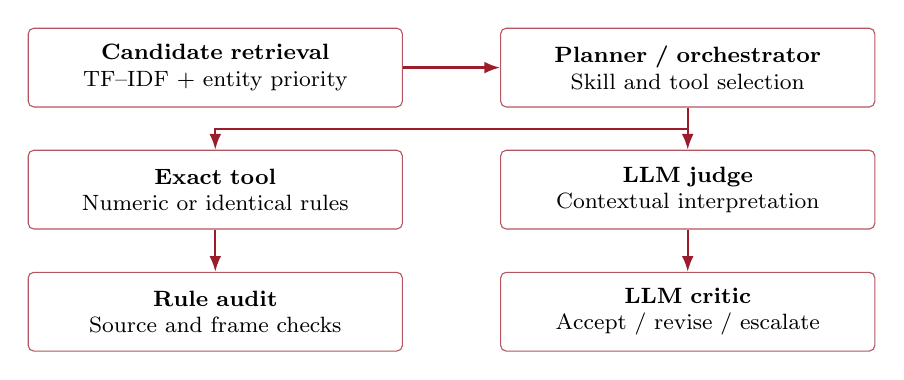
\begin{tikzpicture}[
 font=\footnotesize,
 agentbox/.style={draw=wine!75,fill=white,rounded corners=2pt,align=center,
 text width=4.4cm,minimum height=1cm,inner sep=5pt},
 flow/.style={-{Latex[length=2mm]},draw=wine,line width=.8pt}
]
\node[agentbox] (retrieve) at (0,0) {\textbf{Candidate retrieval}\\TF--IDF + entity priority};
\node[agentbox] (plan) at (6,0) {\textbf{Planner / orchestrator}\\Skill and tool selection};
\node[agentbox] (exact) at (0,-1.55) {\textbf{Exact tool}\\Numeric or identical rules};
\node[agentbox] (judge) at (6,-1.55) {\textbf{LLM judge}\\Contextual interpretation};
\node[agentbox] (rulecritic) at (0,-3.1) {\textbf{Rule audit}\\Source and frame checks};
\node[agentbox] (critic) at (6,-3.1) {\textbf{LLM critic}\\Accept / revise / escalate};
\draw[flow] (retrieve) -- (plan);
\draw[flow] (plan.south) -- (6,-.78) -- (0,-.78) -- (exact.north);
\draw[flow] (plan) -- (judge);
\draw[flow] (exact) -- (rulecritic);
\draw[flow] (judge) -- (critic);
\end{tikzpicture}
\par\vspace{.6em}
\textbf{Outcome:} an evidence-supported proposal or an unresolved case for human review.
\par\vspace{.4em}
{\small The orchestrator allows one revision, then finalizes or escalates. Retrieval similarity alone never supplies a clinical label.}
\end{frame}

\begin{frame}{Skills, tools and hooks give the agents boundaries}
\begin{tabularx}{\textwidth}{@{}p{.18\textwidth}Y@{}}
\toprule
Component & Role in the working system\\\midrule
Skills & Versioned instructions for numeric comparison, clinical context and source problems. The planner selects a skill.\\
Tools & Inspect the comparison frame, compare supported constraints and collect source citations. Only permitted tools run.\\
Hooks & Validate inputs and exact source quotes, check limits and cancellation, and gate the final result.\\
Orchestrator & Coordinates tool calls, judge, critic and revision within pair, call and time limits.\\\bottomrule
\end{tabularx}
\gap
\textbf{Clinician-facing output:} source excerpts, rationale, critic feedback, executed trace and saved reviewer decisions.
\gap
{\small Contextual judge and critic use separate prompts with the configured LLM (currently GPT-4o mini). Agreement does not establish clinical correctness.}
\end{frame}

\begin{frame}{Retrieval progress and the model still to train}
\begin{columns}[T,onlytextwidth]
\column{.48\textwidth}
\textbf{Implemented by Jiatong}
\begin{itemize}
\item TF--IDF, MPNet and BioLORD retrieval backends.
\item Cross-trial ranking with a shared neighbor format.
\item Provisional runs on 200 criteria across 100 trials.
\end{itemize}
\column{.48\textwidth}
\textbf{Current local demo}
\begin{itemize}
\item Uses the original TF--IDF encoder as the temporary retriever.
\item Exact tools and LLM reasoning assign relationships.
\item Dense baseline integration awaits the teammate PR.
\end{itemize}
\end{columns}
\gap
\textbf{Next model step:} use reviewed comparisons to train and evaluate a clinically informed encoder and directional relationship component.
\gap
Clinical retrieval quality and improvement over the baselines are not yet measured.
\end{frame}

\begin{frame}{Where TriAlign fits among eligibility systems}
\textbf{TriAlign:} compare criteria across two trials and explain equivalence,
restrictiveness, overlap or uncertainty using source evidence.
\gap
{\footnotesize
\begin{tabularx}{\textwidth}{@{}p{.20\textwidth}p{.28\textwidth}Y@{}}
\toprule
System & Primary task & Planned connection to TriAlign\\\midrule
\href{https://github.com/ncbi-nlp/TrialGPT}{TrialGPT} & Patient-to-trial matching & Adapt evidence-based judgments to common criterion pairs.\\
\href{https://arxiv.org/abs/2604.02678v1}{EligMeta} & Evidence synthesis & Compare eligibility alignment and LLM / deterministic execution.\\
\href{https://aclanthology.org/2024.findings-eacl.149/}{CReSE} & Criterion recommendation & Compare embeddings if reproducible artifacts permit.\\
\href{https://arxiv.org/abs/2604.08849v4}{SatIR} / \href{https://arxiv.org/abs/2609.03366v1}{VERDICT} & Logical matching and rationales & Study consistency, explicit assumptions and explanation faithfulness.\\
\href{https://aclanthology.org/2025.findings-acl.491/}{EC-RAFT} & Criterion generation & Adjacent authoring work, outside the direct benchmark.\\\bottomrule
\end{tabularx}
}
\gap
{\footnotesize \textbf{Planned evaluation:} common cases and evidence where tasks align. Compare labels, evidence support, abstention, latency and cost. No external-system results yet.}
\end{frame}

\begin{frame}{What the prototype resolves and where it stops}
{\small Trial A: NCT05379712 \qquad Trial B: NCT02769832}
\gap
\begin{columns}[T,onlytextwidth]
\column{.47\textwidth}
\textbf{Supported age comparison}
\gap
A: ``$\geq18$ years of age''\\[4pt]
B: ``Age $\geq18$ years old, both male and female''
\gap
\status{Equivalent in the age frame.}
\gap
The exact tool compares allowed ages. This does not establish equivalence of the whole trials.
\column{.49\textwidth}
\textbf{Consent comparison needing review}
\gap
A: ability to read, understand and sign consent.\\[4pt]
B: willingness and ability to sign consent.
\gap
\status{No supported final label in the saved run.}
\gap
The source-quote check rejected the model's citations. The case remains unresolved for review.
\end{columns}
\gap
{\small These are observed prototype outcomes. Shared consent wording does not establish equivalence of literacy, understanding and willingness.}
\end{frame}

\begin{frame}{Current challenges and limitations}
\begin{itemize}
\item Clinical interpretation can fail on timing, exceptions, negation and parent/child scope.
\item Judge and critic can share mistakes. Human review remains necessary.
\item No retrieved candidate does not prove that a requirement is absent.
\item Independent clinical evaluation, final family-aware splits and calibrated uncertainty remain pending.
\item Dense baseline integration and fine-tuning remain ahead.
\end{itemize}
\gap
The UI runs locally. Contextual model calls still need network access and have API costs and latency.
\end{frame}

\begin{frame}{Next steps before the final presentation}
\begin{tabularx}{\textwidth}{@{}p{.18\textwidth}Y@{}}
\toprule
Owner & Deliverable\\\midrule
Jonathan & Finish review of development comparisons and source ambiguities. Finalize family-aware evaluation partitions.\\
Jiatong & Submit the retrieval PR, integrate MPNet/BioLORD and record reproducible model revisions.\\
Together & Evaluate retrieval and relationship predictions against reviewed labels. Analyze errors and critic behavior.\\
Together & Improve and rehearse the local interface, including evidence inspection and reviewer corrections.\\
Together & Train the clinical encoder once labels and evaluation partitions are ready, then compare with frozen baselines.\\\bottomrule
\end{tabularx}
\gap
Longer term: let Modern AutoCrit and TriAlign run separately or together in one tool.
\end{frame}

\begin{frame}{Questions and feedback}
\Large
Which differences matter most when comparing two trial protocols?
\gap
What evidence would help you trust or correct a proposed relationship?
\gap
When should the system stop and ask for clinical review?
\end{frame}

\end{document}
